Wolfenstein 3D is a game that needs little introduction. It is THE game that back in the days layed down the fundations of the First Person Shooter genre so DOOM could build a temple on top of it.\\
\\
Released in May 1992, it immediatly achieved legendary status. Universaly acclaimed, the beautiful graphics, crisp digitalized sounds, engaging musics and oustanging game design made the game engine sing. Within a year more than 100,000 units were sold bringing game and a little bit of fortune to the game studio producing it: id Software.\\
\\
Fans were so dedicated they reverse engineered as much as possible. Within a few months, the assets format was well known and people started to released modified version (mods) with different graphics, sounds, music and maps. But the 3D engine internals remained mostly unknown.\\
\\
As the money maker, supposed to outperform competition, a game engine is usually a closely guarded secret. So it came at great surprise when on July 21, 1995 id Software decided to release the full source code to the public.
\\

As it turns out, it happened after many internal discution and struggle within the team. In the end, they did the Right Thing. 

 \begin{fancyquotes}
   Programming is not a zero-sum game. Teaching something to a fellow programmer doesn't take it away from you. I'm happy to share what I can, because I'm in it for the love of programming.\\
   \\
\textbf{John Carmack - Programmer}
 \end{fancyquotes}
\\
\\
Releasing the source code, allowing enthousiast to contribute and learned built an aura around id Software and their programmers. With access to the source programmers all around the world were able to learn. I was amond them and I remember vividly the increasing excitment of reading the source: The more I understood about the software, the more I realized how incredibly difficult the hardware was to tame.\\
\\
It may come at a surprise to read this. Plotting the power of the CPU of the system of the time place a standard PC (386 SX 16Mhz) far above the best gaming system (Figure \ref{fig:game_console_vs_PC}).\\
\\
\begin{figure}[H]
\centering
  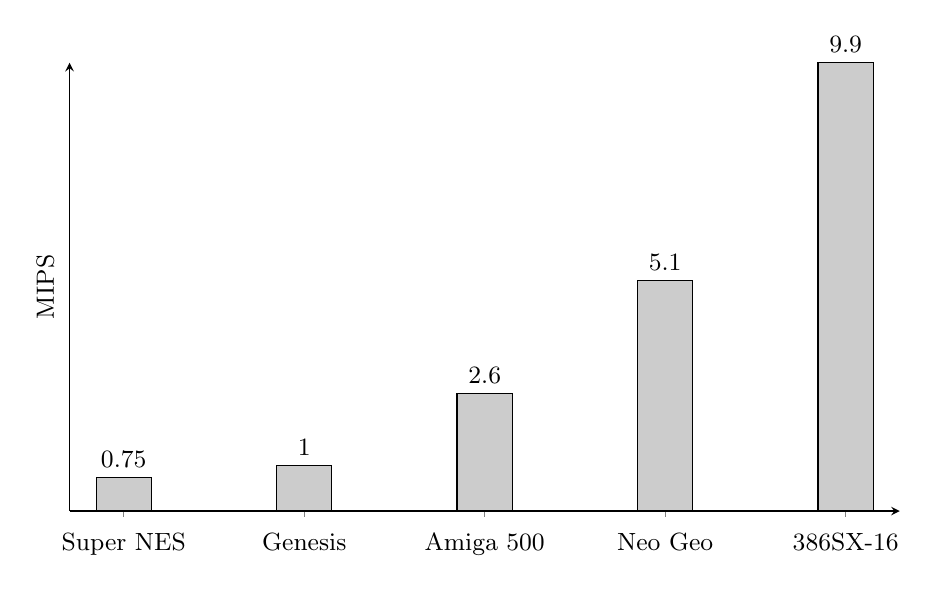
\begin{tikzpicture}[font=\small]
    \begin{axis}[
      width=1.0\textwidth,
      height=0.6\textwidth,
      ybar=6pt,
      bar width=20pt,
      ylabel={MIPS},
      ymin=0,
      ytick=\empty,
      xtick=data,
      axis x line=bottom,
      axis y line=left,
      enlarge x limits=0.075,
      symbolic x coords={Super NES,Genesis,Amiga 500,Neo Geo,386SX-16},
      xticklabel style={anchor=base,yshift=-\baselineskip},
      nodes near coords={\pgfmathprintnumber\pgfplotspointmeta}
    ]
      \addplot[fill=black!20,draw=black] coordinates {
        (Super NES,0.75)
        (Genesis,1)
        (Amiga 500,2.6)
        (Neo Geo,5.1)
        (386SX-16,9.9)
      };
    \end{axis}
    
   \end{tikzpicture}
   \caption{Game Console Vs PC.} \label{fig:game_console_vs_PC}
 \end{figure}

But game console were specifically build and designed to produce 60 frames per seconds animations. Among other things they all had co-processors powering a tile-based system. PCs were sitting on the antipod: Built around a single processor and a framebuffer (a structure were every pixel has to be populated individually) the machine was not designed for gaming, it was intended to crunch integers and display static content.\\
\\
This is where the root of my admiration for Wolfenstein 3D lies: id Software achieved the unthinkable by building a game engine able to display pseudo 3D at 30 frames per seconds on an IBM PC.\\
\\
This book "raison d'etre" is to expose how limited and unwelcoming the hardware was and how the software managed to not only workaround the many limitations but sometimes managed to turn them into an advantage.\\
\\
I saw beauty in how the hardware was repurposed of used in unexpected ways. You had to be driven by passion to program games on those things. Even the engineers building the the hardware would have said that what id Software was trying to achieve was not what the machines were meant to do. This is where the true beauty of Wolfenstein 3D is: For every obstacles, the id Software team found a way to not only circumvent the limitations but often turn them into advantages.

\bigskip

 \textbf{\underline{Disclaimer :}} The description that follows is technical and will appeal mostly to programmers. If you are more into the human aspect of game programming I would recommend instead to read David Kushner’s chef d’oeuvre: “Masters of Doom: How Two Guys Created an Empire and Transformed Pop Culture”.
This book tries to give a detailed story of how Wolfenstein 3D was done. It is divided in three parts reviewing the hardware, the team and the software.